\chapter{User Experience Evolution}

\section{Early Computers}
Computers and how we use them have changed dramatically as each generation is introduced to faster and better machines. How we interact with computers has changed drastically since the first electronic computers in the mid-1900s.

\begin{wrapfigure}{r}{0.5\textwidth}
  \begin{center}
    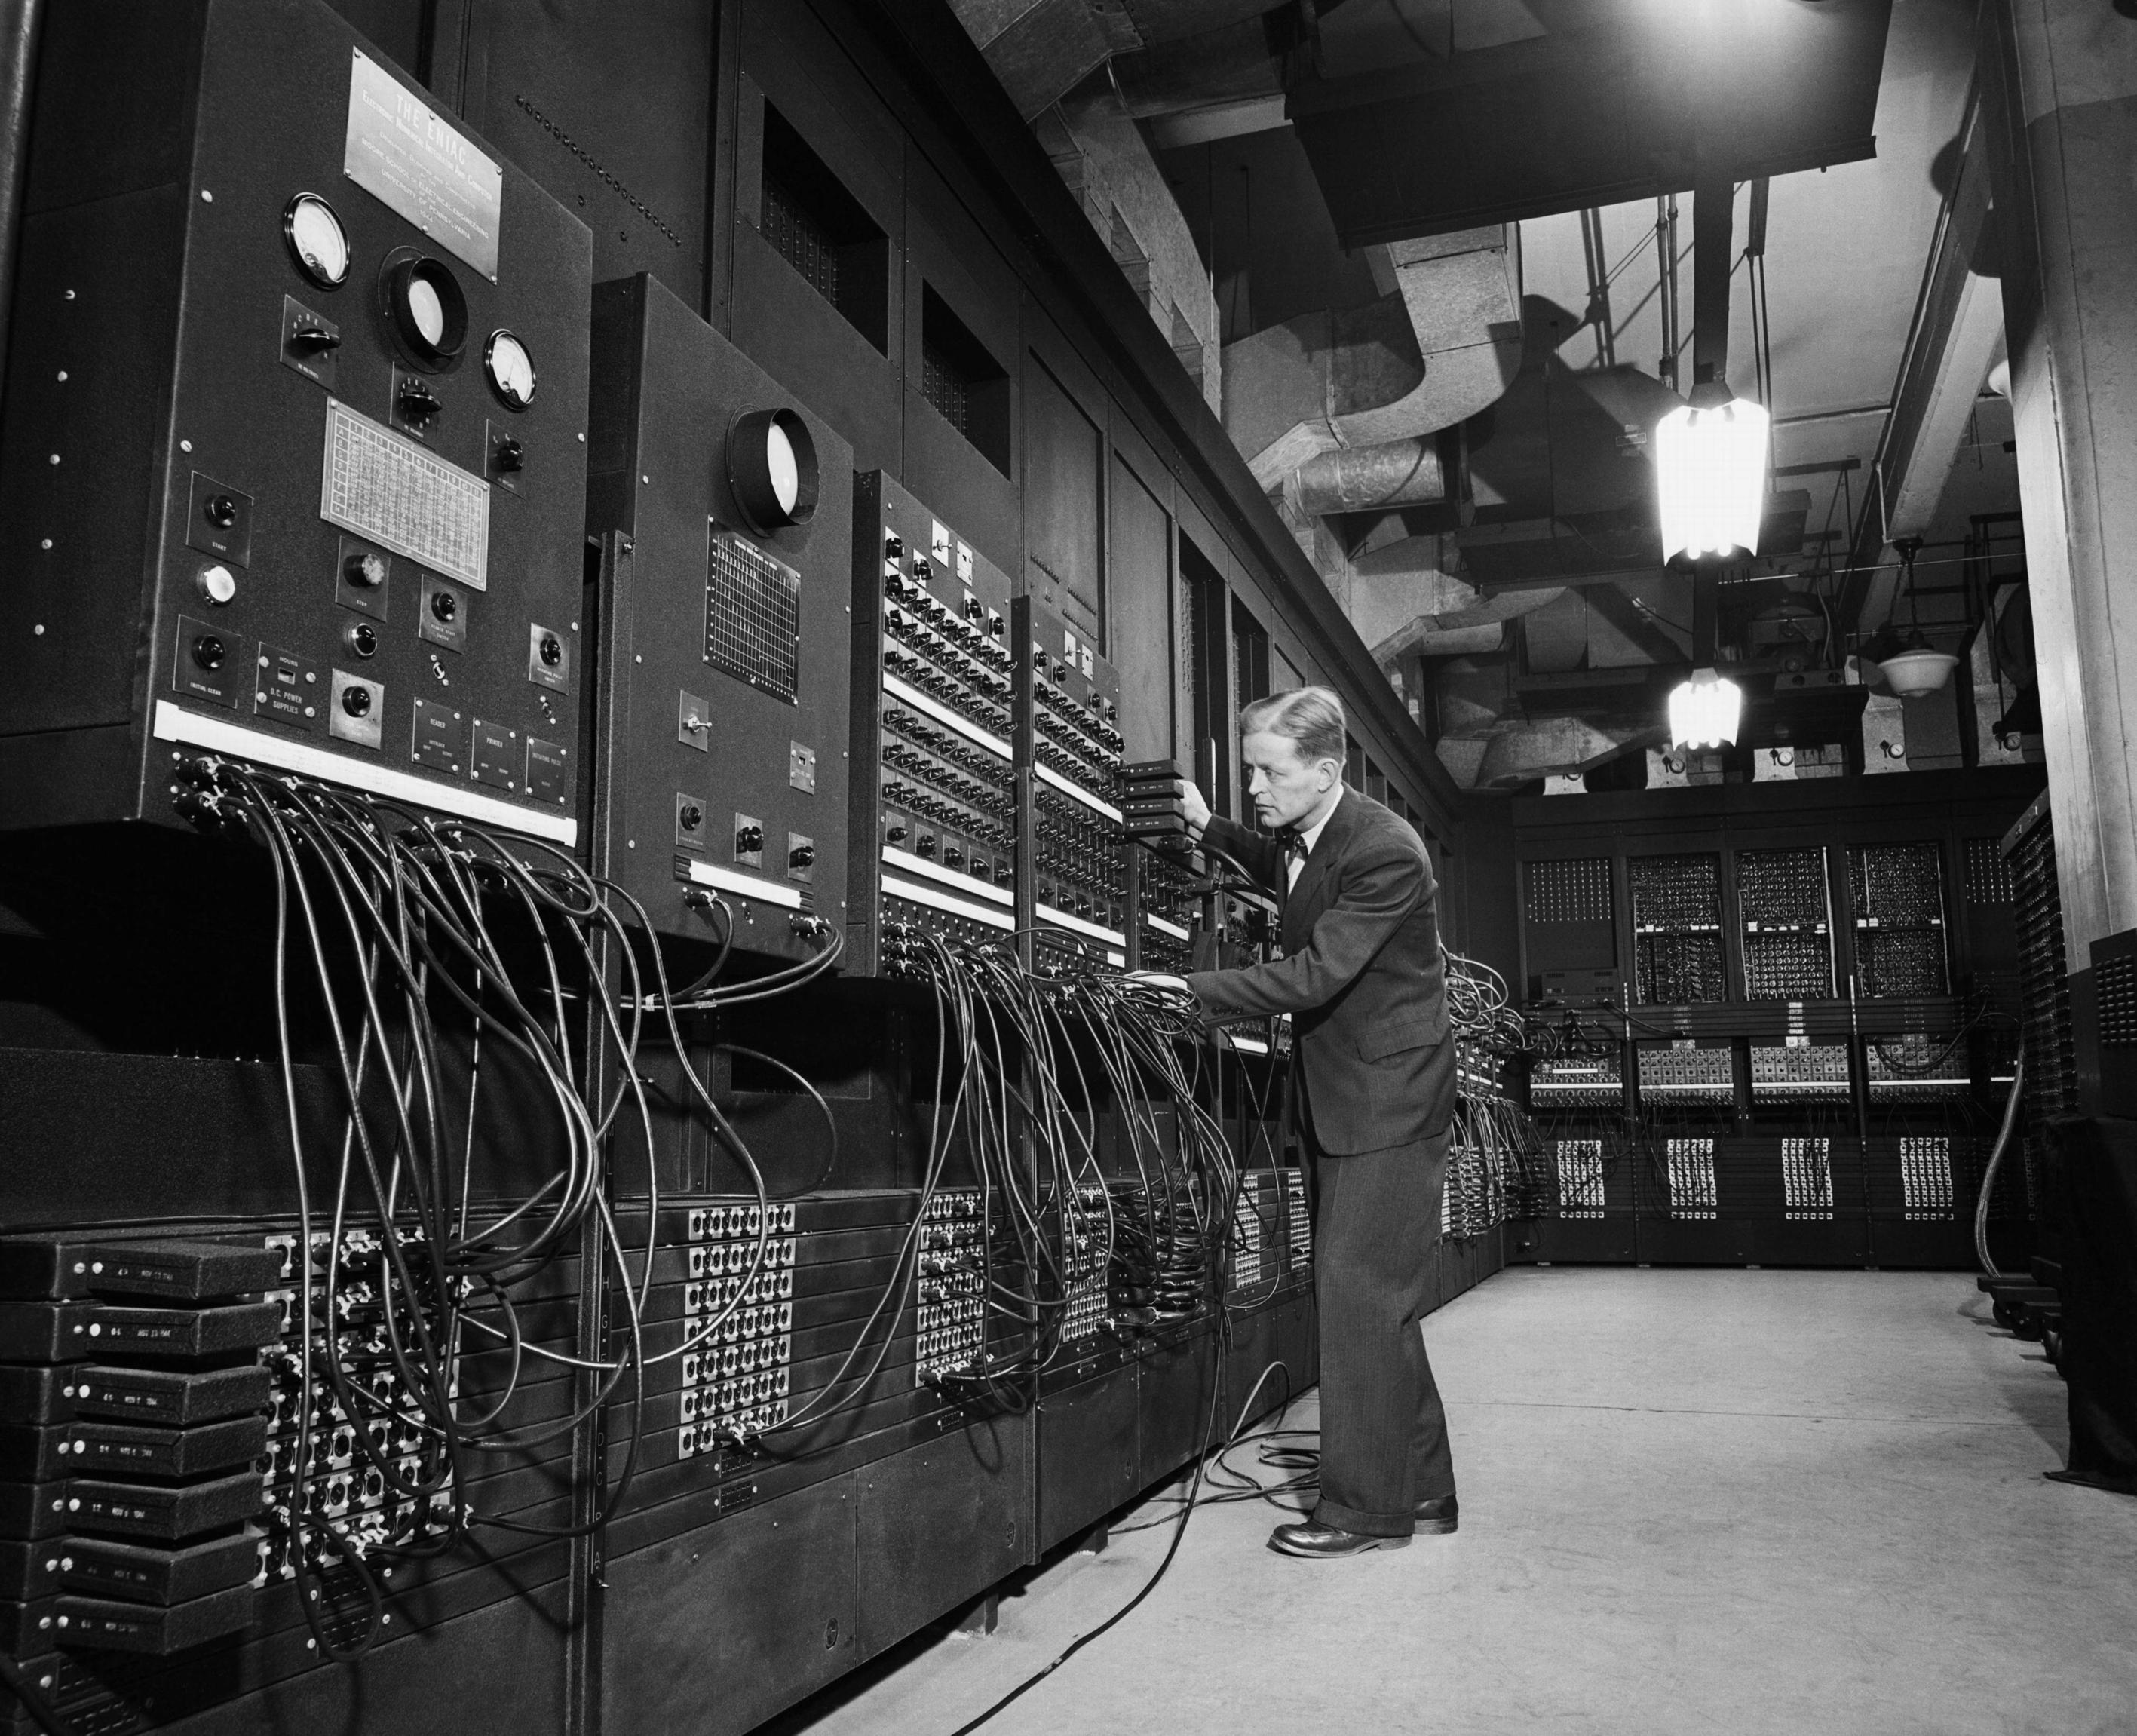
\includegraphics[width=0.48\textwidth]{img/eniac.jpg}
  \end{center}
  \caption{ENIAC}
\end{wrapfigure}

Early electronic computers such as the ENIAC (Electronic Numerical Integrator and Computer). \cite{eniac} The ENIAC was the first general purpose computer, this meant it could solve many problems as it could be programmed. The ENIAC was the first real step in user interaction with a computer, although the user had to have knowledge of the machine first, they could still operate it using over 3,000 switches and wires which could change how the machine made calculations. \cite{eniac} Although a primitive method of user interaction with a machine, it was the first 'modern' computer which the user had some control over its operation and change its operation by interaction.

Moving on from the ENIAC new computers were built with observations on how to improve over the ENIAC. Machines like the Manchester Baby \cite{manchesterbaby} allowed programs to be saved which was a huge leap in user intractable computers. Once a program was created by a programmer of the machine they could be saved and used again at a later date. This was a big step over the ENIAC where it took time to reprogram the machine each time they wanted to compute a specific task.

\section{}
